% !TeX root = 00General.tex
\thispagestyle{standard}
\pagestyle{standard}
\chapter{Ausgangslage}

Im Auftrag einer Firma, die vor kurzer Zeit durch einen Netzwerkausfall erheblichen Schaden erlitten hat, soll das Firmennetzwerk ausfallsicherer gemacht werden. Eine Bedingung ist, dass keine neue Hardware angeschafft werden soll. Abbildung \ref{img:Ausgangslage} zeigt den derzeitigen Netzwerkaufbau.

\begin{figure}[H]
	\centering
	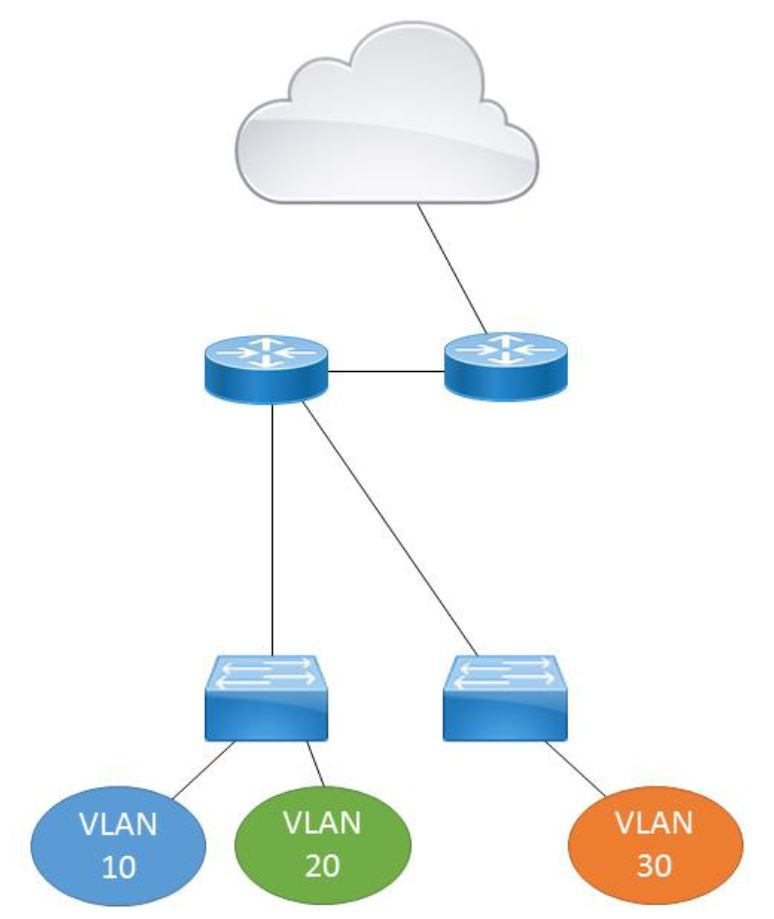
\includegraphics[width=0.9\textwidth]{img/Ausgangslage.JPG}
	\caption{Ausgangslage Netzwerktopologie}
	\label{img:Ausgangslage}
\end{figure}

\chapter{Netzwerkplanung}

Das zu planende Netzwerk soll im Hinblick auf Netzzuverlässigkeit optimiert werden. Dazu fordert der Kunde eine redundante Internetanbindung. Diese wird mit einer seriellen Verbindung zu \ac{ISP} 1, durch Punkt 1 in Abbildung \ref{img:Netzwerkplanung} dargestellt, erreicht. 

\begin{figure}[H]
	\centering
	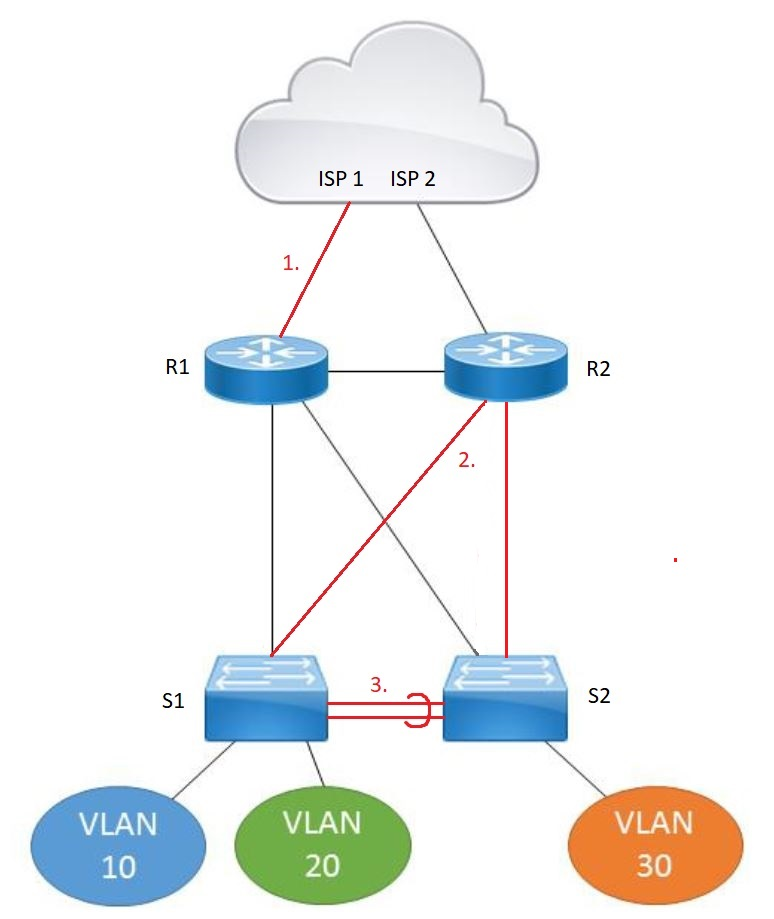
\includegraphics[width=0.9\textwidth]{img/Planung_neu.JPG}
	\caption{Planung des ausfallsicheren Netzwerks}
	\label{img:Netzwerkplanung}
\end{figure}

Durch die in Punkt 2 ergänzten Verbindungen wird eine Ausfallsicherheit für Router 1 und Router 2 erzeugt. Es wird dadurch möglich, dass im Falle eines Ausfalls von Router 1 denoch Verbindungen von \ac{VLAN} 10 in \ac{VLAN} 30 aufgebaut werden können.

Punkt 3 in Abbildung \ref{img:Netzwerkplanung} zeigt die Implementierung von EtherChannel. Werden in nächster Zeit weitere \ac{VLAN}s an verschiedene Router gehängt, so entsteht durch EtherChannel eine Bandbreitenerhöhung bzw. Load-Balancing zwischen z.B. \ac{VLAN} 10 an Switch 1 und Switch 2. Des weiteren hat EtherChannel einen sogenannten "Fail-Over Mode". Die EtherChannel Technologie verteilt die Last automatisch auf die verbleibenden Links.

\textbf{\ac{VLAN} \ac{IP} Adressen Bereich:} 

\begin{itemize}  
\item VLAN 10: 192.168.5.0/24
\item VLAN 20: 192.168.15.0/24
\item VLAN 30: 192.168.25.0/24
\end{itemize}

\chapter{Konfiguration des Netzwerks}

\section{Switches}

Um nun die EtherChannel Technologie zu realisieren wurden die Ports "FastEthernet 23 und 24" verwendet. Diese werden als sogenannte "Trunk Links" konfiguriert.

\lstset{escapeinside={\%*}{*)},numbers=left}%oder numbers=left
\begin{lstlisting}[caption={Setting EtherChannel on a switch},label={lst:etherchannel},language={}]
interface FastEthernet0/24
 switchport trunk allowed vlan 10,20,30
 switchport mode trunk
 channel-protocol lacp
 channel-group 1 mode active
\end{lstlisting}

Des weiteren wurden die verschiedenen \ac{VLAN}s, die auf den jeweiligen Switches hängen, konfiguriert. Im Listing 3.2 werden zwei solchen Konfigurationen dargestellt.

\lstset{escapeinside={\%*}{*)},numbers=left}%oder numbers=left
\begin{lstlisting}[caption={VLAN Konfiguration auf Switch 1},label={lst:etherchannel},language={}]
interface Vlan10
 ip address 192.168.5.254 255.255.255.0
!
interface Vlan20
 ip address 192.168.15.254 255.255.255.0

\end{lstlisting}

\section{Router}
Wie im folgenden Listing 3.3 erkennbar, wurden die GigabitEthernet Interfaces (je nach \ac{VLAN}) für die Encapsulation (IEEE 802.1Q) konfiguriert. Für die jeweiligen Standby Gruppen wurden die dazugehörigen IP-Adressen angegeben. 
Diese standby Adressen werden dazu genutzt, um das \ac{HSRP} zu nutzen und eine IP Redundanz abzudecken. Diese soll im Ausfall ("statefull failover") die Funktionalität aufrechterhalten.

\lstset{escapeinside={\%*}{*)},numbers=left}%oder numbers=left
\begin{lstlisting}[caption={Konfiguration auf Router 1},label={lst:routerconfig},language={}]
interface GigabitEthernet0/0.10
 encapsulation dot1Q 10
 ip address 192.168.5.1 255.255.255.0
 standby 1 ip 192.168.5.10
!
interface GigabitEthernet0/0.20
 encapsulation dot1Q 20
 ip address 192.168.15.1 255.255.255.0
 standby 2 ip 192.168.15.10
!
interface GigabitEthernet0/0.30
 encapsulation dot1Q 30
 ip address 192.168.25.1 255.255.255.0
 standby 3 ip 192.168.25.10

\end{lstlisting}

Des weiteren wurde auch \ac{OSPF} genutzt (siehe Listing 3.3), um  den Routern ein schnelles dynamisches Verhalten in Bezug auf die Änderungen in der Netztopologie zu ermöglichen. Durch diese Nutzung optimiert sich das Routing hinsichtlich der Übertragungskosten und kann im Notfall daher nützlich sein.

\lstset{escapeinside={\%*}{*)},numbers=left}%oder numbers=left
\begin{lstlisting}[caption={OSFP Einstellungen auf Router 2},label={lst:ospfsettings},language={}]
router ospf 10
 network 10.10.10.0 0.0.0.255 area 0
 network 172.16.15.0 0.0.0.3 area 0
 network 192.168.25.0 0.0.0.255 area 0

\end{lstlisting}

